\renewcommand{\thesection}{Basic Task}

\newcommand{\upa}{\mathlarger{\uparrow}}
\newcommand{\downa}{\mathlarger{\downarrow}}
\newcommand{\lefta}{\mathlarger{\leftarrow}}
\newcommand{\righta}{\mathlarger{\rightarrow}}

\section{Q Learning}

\subsection{Working Environment and State Transition and Reward Functions}

\begin{figure}[h]
	\begin{subfigure}{.49\textwidth}
		\centering
		\includegraphics[width=170pt,height=125pt,draft]{snow_puzzle_original.png}
		\caption{Original puzzle}
	\end{subfigure}
	\begin{subfigure}{.49\textwidth}
		\centering
		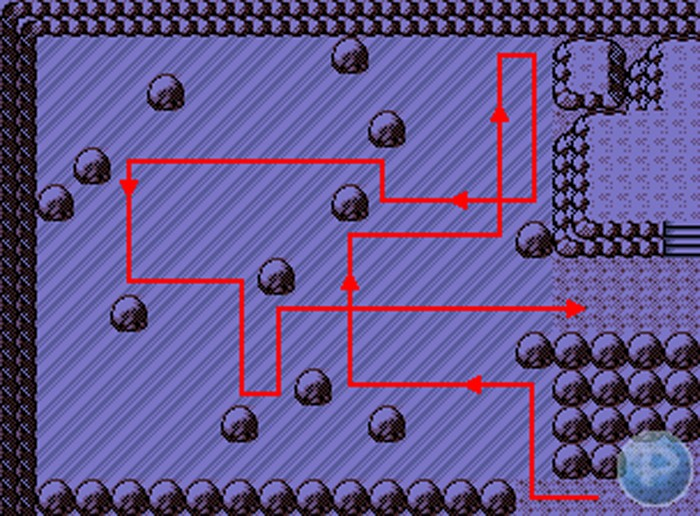
\includegraphics[height=125pt]{snow_2.png}
		\caption{Puzzle solution}
	\end{subfigure}
	\caption{An example of a Pokémon Ice puzzle}
	\label{large_map}
\end{figure}

In this task we present a solver of \emph{Pokémon Ice Puzzles}, a kind of ice puzzle where the player starts at a certain position $s$ and has the objective to reach its objective $e$ in as few steps as possible.

At each turn, the player can do one of four movements: $\{\upa, \downa, \lefta, \righta\}$.
As the environment is ice, when the user walks in any direction is slips on the ice and keeps going on the same direction until hitting a rock or the edge.

\newcommand{\coor}[2]{\left\langle #1, #2 \right\rangle}
\newcommand{\yx}{\coor{y}{x}}
\newcommand{\obs}{\mathcal{O}}
\newcommand{\state}{\mathcal{S}}
\newcommand{\reward}{\mathcal{R}}
The state function $\state$, along with the transition and reward functions $\mathcal{T}$ and $\reward$ can be defined as the following, where $\obs_{\yx}$ is true if and only if there is an obstacle on position $\yx$.
\begin{gather*}
	\state = \yx \qquad \mathcal{D} \in \left\{ \upa, \downa, \lefta, \righta \right\} \\
	\begin{aligned}
		&T_{\yx}\left(\upa\right) &= \coor{t + 1}{x} &&&\text{where } \obs_{\coor{t}{x}} \wedge \neg \obs_{\coor{q}{x}} \forall q \in \left(t, y\right) \\
		&T_{\yx}\left(\downa\right) &= \coor{t - 1}{x} &&&\text{where } \obs_{\coor{t}{x}} \wedge \neg \obs_{\coor{q}{x}} \forall q \in \left(y, t\right) \\
		&T_{\yx}\left(\lefta\right) &= \coor{y}{t + 1} &&&\text{where } \obs_{\coor{y}{t}} \wedge \neg \obs_{\coor{y}{q}} \forall q \in \left(t, x\right) \\
		&T_{\yx}\left(\righta\right) &= \coor{y}{t - 1} &&&\text{where } \obs_{\coor{y}{t}} \wedge \neg \obs_{\coor{y}{q}} \forall q \in \left(x, y\right)
	\end{aligned} \\
	\reward(\yx) = \begin{cases}
		100 & \text{if } e = \yx \\
		0 & \text{otherwise}
	\end{cases}
\end{gather*}

\subsection{Q Function}

This transition function allows us to define an iterative $Q$ function, which should be used to find the objective $Q^\pi$ function.
\begin{gather*}
	s \in \mathcal{S} \qquad a \in \mathcal{D} \\
	Q^{k + 1}(s, a) = \alpha \cdot \left( \reward( T( a, s ) ) + \gamma \cdot \max{Q^k(s, a)} \right) - Q^k(s, a)
\end{gather*}

\newpage{}
The probability next action $a$ is defined depending on the policy used, where $\pi^k(a \mid s)$ represents the probability of choosing action $a$ with state $s$ at point $k$.
\begin{gather*}
	\intertext{\textbf{\textepsilon-Greedy Policy}: choose the best policy with probability $\varepsilon$, randomly otherwise.}
	\pi^k(a \mid s) = 
		(1 - \varepsilon) \cdot \frac{1}{\mathcal{D}} + \varepsilon \cdot \begin{cases}
			1 & \text{if } a = \argmax_{a'} (Q^k(s, a')) \\
			0 & \text{otherwise}
		\end{cases} \\
	\intertext{\textbf{Bellman Policy}: choose policy using the softmax of the Q-value}
	\pi^k(a \mid s) = \frac{e^{Q^k(s, a)}}{\sum_{a' \in \mathcal{D}}{e^{Q^k(s, a')}}}
\end{gather*}

\subsection{Parameter sweep}
To find the best parameters, we run a parameter sweep on the map in \cref{large_map} for each combination of parameters in \cref{param_sweep_params}; this map is large enough to make it suitable for a parameter sweep.

\begin{table}[h]
	\scriptsize
	\centering
	\begin{tabular}{>{\bfseries}r | l l l l}
		\toprule
		Hyperparameter & \multicolumn{4}{c}{Values} \\
		\midrule
		Policy & \multicolumn{4}{l}{\begin{tabular}{l l}$\varepsilon$-Greedy & Bellman\end{tabular}} \\
		$\alpha$ & 0.1 & 0.5 & 0.7 & 0.9 \\
		$\gamma$ & 0.9 & 0.99 && \\
		$\varepsilon$ Decay Rate & 0.75 & 0.9 & 0.99 & \\
		\bottomrule
	\end{tabular}
	\caption{The parameter sweep considered every possible combination of these parameters.}
	\label{param_sweep_params}
\end{table}

Each combination was run 10 times until the Q matrix converged to a precision of $10^{-12}$ and results were averaged.
The final results, which contain the best parameters, can be found in \appendixA{}
Some interesting results can be found in \cref{param_sweep_interesting}.

\begin{table}[h]
	\scriptsize
	\centering
	\begin{tabular}{>{\bfseries}r r l r | r r r r}
		\toprule
		Policy & $\alpha$ & $\gamma$ & $\varepsilon$ Decay &
		E.\ to Conv & Best route & E.\ to Done & E.\ to Best \\
		\midrule
		\rowcolor{YellowGreen}
		\textepsilon{}-Greedy & 0.5  & 0.90  & 0.99 & 139 & 16.00 & 31.80  & 97 \\
		\textepsilon{}-Greedy & 0.9 & 0.90  & 0.90 & 51  & 16.80 & 12.00  & 26 \\
		\midrule
		Bellman & 0.2 & 0.90 & 0.75 & 666  & 16.20 &  82.70 &  224 \\
		Bellman & 0.9 & 0.90 & 0.99 & 126  & 17.40 &  37.30 &   86 \\
		Bellman & 0.7 & 0.90 & 0.75 & 205  & 17.60 &  48.70 &   58 \\
		\bottomrule
	\end{tabular}
	\caption{Some notable results taken from \appendixA{}.}
	\label{param_sweep_interesting}
\end{table}

We can observe the following.
\begin{itemize}
	\item The \textepsilon{}-Greedy policy converges faster and produces a significantly better result.
	\item Generally having high $\varepsilon$ Decay represents better results.
	\item There is a significant correlation between convergence speed and how good the solutions are.
\end{itemize}

We choose the parameter combination that converges the fastest between the ones that \emph{always} found the best solution; that's marked in \colorbox{YellowGreen}{green}.
